%!TEX root = ../Thesis.tex
\section{UserStories \& Use Cases}

\subsection{User Story}

\subsubsection{Niklas Hardes}

Ich als Gamer möchte wissen, welche Spiele am beliebtesten sind, am meisten gespielt werden und infolgedessen für mich am interessantesten sein können.

\subsection{Robert Hesselmann}

Ein erfolgreicher Streamer auf der Livestreaming Plattform Twitch sucht nach neuen Spielen, die er in seinen Livestreams Spielen kann. Um seinen Gewinn zu maximieren sucht er nach einem Spiel zu einem günstigen Preis.

\subsection{Use Case}


\subsection{Robert Hesselmann}

\begin{figure}[hbt]
    \centering
    \begin{minipage}[t]{1\textwidth} % Breite, z.B. 1\textwidth		
        \caption{Use Case Streamer} % Überschrift
        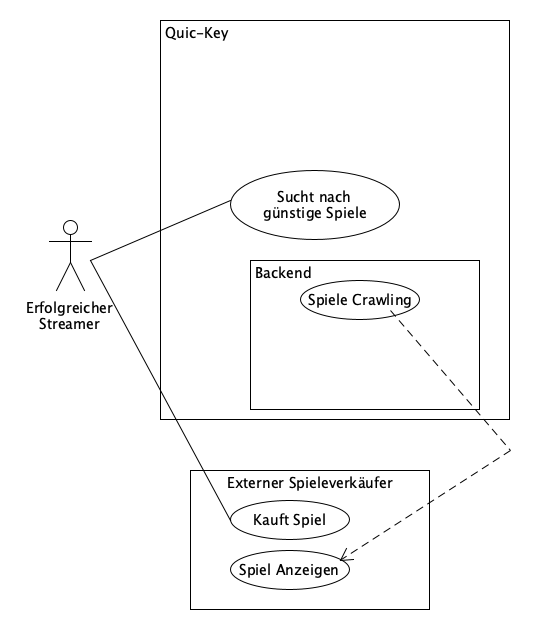
\includegraphics[width=1\textwidth]{img/use_case_streamer.png}\\ % Pfad
        \source{Eigene Darstellung} % Quelle
    \end{minipage}
\end{figure}